\documentclass{aruno-gist}

\usepackage{mylayout}

%% Details of the book
%% ===================

\title{Riflessioni sul Dhammapada}
\subtitle{52 versi dal Dhammapada con i commenti}
\author{Ajahn Munindo}
\date{}
\editionInfo{\textit{Prima edizione}, 10.000 copie, stampato in Malesia, 2013}
\ISBN{978-1-908444-34-9}

\begin{document}

\thispagestyle{empty}
\mbox{}
\pagecolor[gray]{0.7}
\newpage
\thispagestyle{empty}
\pagecolor{white}
\mbox{}
\newpage

%% Frontmatter
%% ===========

\frontmatter*
\pagestyle{empty}

\midsloppy

\cleartorecto
\begin{quotepage}{60mm}
\centering
\itshape
Mirando all'obiettivo della liberazione\\
il saggio abbandona l'oscurit\`{a}\\
e ha cara la luce,\\
si lascia alle spalle\\
la sicurezza meschina\\
e cerca la libert\`{a} dall'attaccamento.\\
Il desiderio di libert\`{a}\\
\`{e} cosa ardua e rara\\
ma il saggio continuer\`{a} a cercare\\
distaccandosi da tutto ci\`{o} che si frappone,\\
purificando il cuore e la mente.

{\smaller Dhammapada strofe 87-88}
\end{quotepage}

\cleartoverso
\begin{quotepage}{80mm}
\centering
\textit{Dedica}\\[0.4\baselineskip]
Vogliamo ringraziare le tante persone che ci hanno sostenuto nella preparazione di questo libro, e in particolare, il gruppo Kataññutā in Malesia, Singapore e Australia, per averne reso possibile la pubblicazione.

\end{quotepage}

\cleartorecto
\thispagestyle{empty}

\vspace*{1em}

{\centering

\soChapter{RIFLESSIONI SUL dHAMMAPADA}\\[0.4\baselineskip]
Volume 2
\vspace*{3\baselineskip}

{\itshape 52 versi dal Dhammapada\\
con i commenti}

\vspace*{2\baselineskip}
di Ajahn Munindo

\vfill

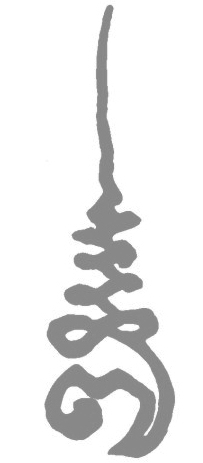
\includegraphics[keepaspectratio, height=17mm]{buddho.jpg}
\vspace*{1.3em}

\soChapter{ARUNO PUBLICATIONS}

}


\cleartoverso
\thispagestyle{empty}
{\copyrightsize\setlength{\parskip}{0.5\baselineskip}\setlength{\parindent}{0em}%
\raggedright%
\shaker\color[gray]{0.3}

\thetitle\\
di \theauthor

Pubblicate da Aruno Publications,\\
Northumberland, Gran Bretagna

Contattare Aruno Publications \href{http://ratanagiri.org.uk/}{www.ratanagiri.org.uk}\\
Questo libro \`{e} scaricabile gratuitamente all'indirizzo\\
\href{http://forestsanghabooks.org/}{www.forestsanghabooks.org}

ISBN \theISBN

Copyright \copyright\ 2013 HARNHAM BUDDHIST MONASTERY TRUST

\textit{Sabbadānaṃ dhammadānaṃ jinati}\\
``Il dono del Dhamma supera tutti i doni''

Foto di copertina di Chinch Gryniewicz\\
\href{http://chinch-gryniewicz.com}{www.chinch-gryniewicz.com}

{\tiny

Attribuzione - Non commerciale - Non opere derivate 3.0 Unported\\
\href{http://creativecommons.org/licenses/by-nc-nd/3.0/}{http://creativecommons.org/licenses/by-nc-nd/3.0/}

Consultare pagina \pageref{copyright-details} per maggiori dettagli su diritti e restrizioni relativi a questa licenza.

Prodotto con {\fontfamily{cms}\selectfont\LaTeX} typesetting system.

\theEditionInfo

}}



\chapterstyle{frontmatter}

\chapter{Prefazione}

Il secondo volume delle \emph{Riflessioni sul Dhammapada} fa seguito al primo, pubblicato nel 2009. Anche questa volta, il volume comprende una selezione di 52 citazioni da \emph{Un Dhammapada per la contemplazione} (2006) e i relativi commenti. Citazioni e commenti sono stati precedentemente pubblicati come messaggi mail spediti a ogni luna nuova e luna piena ai membri della nostra comunit\`{a} per corrispondenza on-line del Dhammasakaccha, che ha attualmente circa 600 partecipanti. Se desiderate ricevere queste mail visitate:

\vspace*{0.2\baselineskip}
{\centering
www.ratanagiri.org.uk/dhammapada-reflections/

}
\vspace*{0.2\baselineskip}

Ancora una volta, sono in debito verso le tante persone che hanno dato una mano nella preparazione di questo materiale. Per i versi del Dhammapada, ho consultato molte autorevoli versioni. In particolare, ho utilizzato il lavoro del Ven. Narada Thera (B.M.S. 1978), Ven. Ananda Maitreya Thera (lotsawa 1988), Daw Mya Tin e dei redattori della Burmese Pitaka Association (1987) e di Ajahn Thanissaro. Per le storie tramandate associate con i versi mi sono rivolto  a www.tipitaka.net.

Ron Lumsden e Jayasiri Lewis hanno generosamente offerto il loro tempo e le loro capacit\`{a} per rivedere i testi.

Che le benedizioni che possono sorgere da questa raccolta siano condivise con tutti coloro che sono stati coinvolti nella sua produzione e sponsorizzazione. Che tutti quelli che cercano la via possano trovarla e possano sperimentare, alla sua conclusione, la libert\`{a}. Che tutti gli esseri cerchino la via.


{\par\raggedleft
Bhikkhu Munindo\\
Aruna Ratanagiri Buddhist Monastery\\
Northumberland, Gran Bretagna
\par}



%% Main matter
%% ===========

\mainmatter*

\cleartorecto
\thispagestyle{empty}
{\centering

\vspace*{0.6\textheight}
{\chapNameFont\LARGE\color{chaptitle}\soChapter{Riflessioni sul Dhammapada}}

}

\setcounter{chapter}{0}
\setcounter{page}{1}
\pagestyle{normalpage}
\chapterstyle{mainmatter}

\setlength{\parskip}{0.6\baselineskip}
\setlength{\parindent}{0pt}


%% == 1 ==

\begin{dhpVerse}{85}
\label{dhp-85}
Quelli che raggiungono l'altra sponda sono pochi.\\
I più vagano avanti e indietro,\\
senza fine su questa sponda\\
non arrischiandosi al viaggio.
\end{dhpVerse}

\begin{dhpRefl}
Non \`{e} in realt\`{a} possibile immaginare qualcosa di veramente nuovo. Quasi tutto quello che pensiamo \`{e} un riassetto del passato. Abbiamo bisogno di un approccio decisamente nuovo se il nostro obbiettivo \`{e} `l'oltre', la libert\`{a} dalla sofferenza. La prevedibilit\`{a} di ci\`{o} che ci \`{e} familiare ci fa sentire al sicuro, anche se \`{e} monotona. Questo \`{e} il nostro incessante oscillare avanti e indietro. \`{E} così che viviamo con l'attaccamento. Come sarebbe se non ci aggrappassimo, se avessimo fiducia nella consapevolezza qui e ora, permeata dal Dhamma? Ci vuole coraggio per lasciar andare il familiare e aprirsi al non conosciuto. L'impegno ai precetti etici e l'addestramento alla presenza sono i nostri protettori. Con questo assetto, possiamo avere il coraggio di intraprendere il nuovo viaggio.
\end{dhpRefl}

%% == 2 ==

\begin{dhpVerse}{194}
\label{dhp-194}
Benedetta \`{e} la nascita di un Buddha\\
benedetta la rivelazione del Dhamma\\
benedetta l'armonia del Sangha\\
beata \`{e} la melodiosa comunione.
\end{dhpVerse}

\begin{dhpRefl}
L'armonia \`{e} una piacevole risonanza che nasce da diversi elementi: note suonate su uno strumento, colori combinati in un'immagine, opinioni condivise in un dialogo. La diversit\`{a} non \`{e} di per s\'{e} un ostacolo all'armonia e alla concordia. In effetti, il contrasto pu\`{o} arricchire e rendere più profonda l'esperienza. Vivendo con consapevolezza impariamo dove risiede il potenziale della bellezza. Anche il disequilibrio ha una sua bellezza se c'\`{e} armonia; saggezza, abilit\`{a} e sensibilit\`{a} si uniscono e la bellezza si manifesta. Questa \`{e} una rara benedizione.
\end{dhpRefl}

%% == 3 ==

\begin{dhpVerse}{202}
\label{dhp-202}
Non c'\`{e} fuoco pari al desiderio\\
n\'{e} malattia peggiore dell'odio\\
n\'{e} pena che opprima come l'attaccamento\\
n\'{e} gioia pari alla pace della libert\`{a}.
\end{dhpVerse}

\begin{dhpRefl}
Come restare mirati sul sentiero che conduce alla chiarezza e alla pace incrollabile? Avidit\`{a}, avversione e confusione distorcono il nostro pensiero. La brama pu\`{o} sembrare attraente; siamo attirati nel suo vortice. L'odio pu\`{o} sembrare attraente; ci sentiamo spinti a fare il male. L'attaccamento ha radici nella falsa credenza che aggrapparci ci renda più felici. In verit\`{a}, la brama brucia, l'odio intralcia l'intelligenza, e gli attaccamenti rovinano quel che c'\`{e} di bello nella vita. Possiamo cominciare a capire questa verit\`{a} da noi stessi quando addestriamo l'attenzione a vedere attraverso l'apparenza esterna delle cose. Una comprensione più profonda di questi tre veleni ci incoraggia a ritrarci dal seguire i loro impulsi. Questa \`{e} la comprensione che conduce alla liberazione.
\end{dhpRefl}

%% == 4 ==

\begin{dhpVerse}{302}
\label{dhp-302}
E' difficile vivere\\
la vita della rinuncia:\\
raro \`{e} saperne apprezzare\\
le sfide.\\
Ma \`{e} anche difficile vivere\\
la vita del capofamiglia:\\
fa soffrire\\
stare con quelli\\
per cui non si sente amicizia.\\
Vagare senza impegno\\
porta sempre a difficolt\`{a}.\\
Perch\'{e} non rinunciare\\
all'illusorio inseguimento del dolore?
\end{dhpVerse}

\begin{dhpRefl}
Il Buddha rivolse queste parole a un monaco che indulgeva in ingannevoli sensi di auto-commiserazione: ``Sicuramente nessuno sta vivendo una situazione difficile quanto la mia''. Per sua fortuna, il monaco ricevette una saggia riflessione nel modo giusto al momento giusto e riuscì così a vedere quel che stava facendo e a lasciar andare. Quando non siamo attenti nel momento presente, tendiamo a incolpare la cattiva sorte fuori di noi. Oppure biasimiamo noi stessi, interiormente.  In entrambi i casi, accresciamo il dolore dimenticando di espandere la consapevolezza e di accogliere pienamente la sofferenza. La sofferenza \`{e} la giusta risposta al nostro opporre resistenza alla realt\`{a}. Se non ci attacchiamo, non soffriamo. La sofferenza \`{e} un messaggio. Non \`{e} qualcosa che sta andando nel verso sbagliato. Non dobbiamo liberarci dalla sofferenza, dobbiamo ascoltarla.
\end{dhpRefl}

%% == 5 ==

\begin{dhpVerse}{111}
\label{dhp-111}
Un solo giorno vissuto\\
con chiara intenzione e saggezza\\
ha più valore di cento anni\\
privi di disciplina\\
e di manifesta saggezza.
\end{dhpVerse}

\begin{dhpRefl}
Il più bel dono che possiamo offrire al Buddha \`{e} di vivere con saggezza. Tutti noi sappiamo quali sono le conseguenze di una vita basata sulle nostre preferenze: ci sentiamo divisi, non interi. Quando le condizioni convergono nel creare circostanze piacevoli ci smarriamo nella felicit\`{a} raggiunta; quando le condizioni diventano sgradevoli ci disperiamo per quel che abbiamo perduto. La saggezza `vede' sia il guadagno che la perdita, la saggezza sostiene la consapevolezza che ci rende liberi.
\end{dhpRefl}

%% == 6 ==

\begin{dhpVerse}{24}
\label{dhp-24}
Chi spende tutta la sua energia\\
nel percorrere la Via,\\
chi \`{e} puro e sollecito nell'impegno\\
raccolto e onesto nel comportamento,\\
vede accrescere in s\'{e} l'esultanza.
\end{dhpVerse}

\begin{dhpRefl}
Il sentiero del Buddha verso la radiosit\`{a} passa dal lasciar andare. Veniamo incoraggiati a considerare le cose con cura e con tutta la nostra energia fino a penetrare nella loro vera natura, incertezza, instabilit\`{a}, impermanenza. Ci addestriamo a lasciar andare con una comprensione che nasce dall'investigazione, non dal rifiuto o dalla negazione. Esiste anche un sentiero ingannevole della pratica che conduce alla radiosit\`{a} che nasce non dal lasciar andare, ma dall'attaccamento alle opinioni. Aggrapparsi fermamente a idee e sensazioni di essere nel giusto pu\`{o} procurare un forte senso di auto-importanza. C'\`{e} energia, entusiasmo, convinzione. Ma seguire questo sentiero porta a divisione e disarmonia. Se il nostro sforzo \`{e} in accordo con la realt\`{a} c'\`{e} un'interiore contentezza che irraggia benessere.
\end{dhpRefl}

%% == 7 ==

\begin{dhpVerse}{384}
\label{dhp-384}
Le catene di ogni schiavitù si spezzano\\
per chi vede chiaramente\\
e sa bene cosa  siano\\
concentrazione e visione intuitiva.
\end{dhpVerse}

\begin{dhpRefl}
  Un visitatore del monastero chiese all'insegnate di meditazione Venerabile Ajahn Chah come si possa praticare la meditazione di concentrazione (\emph{samādhi}) quando in realt\`{a} non c'\`{e} un s\'{e}. Il maestro spieg\`{o} che quando sviluppiamo la concentrazione, lavoriamo con un s\'{e}. Quando sviluppiamo l'intuizione profonda (\emph{vipassanā}), lavoriamo con il non-s\'{e}. Quindi quando veramente conosciamo lo stato delle cose, siamo al di l\`{a} sia del s\'{e} che del non-s\'{e}. 
\end{dhpRefl}

%% == 8 ==

\begin{dhpVerse}{201}
\label{dhp-201}
La vittoria porta all'odio\\
perch\'{e} gli sconfitti soffrono.\\
Chi \`{e} in pace vive lieto\\
al di l\`{a} di vittoria e sconfitta.
\end{dhpVerse}

\begin{dhpRefl}
Chi vive al di l\`{a} di vittoria e sconfitta \`{e} definito `in pace' non perch\'{e} sia privo di sentimenti. Non \`{e} `al di l\`{a}' perch\'{e} \`{e} sfuggito alle sensazioni di dolore e di perdita, ma perch\'{e} \`{e} sfuggito al raggiro del s\'{e}. Il s\'{e} \`{e} come un arcobaleno. Da lontano sembra reale e solido, ma appena vi avvicinate, sembra meno solido. Se ci aggrappiamo troppo saldamente al senso del s\'{e}, ci perdiamo in opinioni riguardo a cosa ci renda felici. Crediamo che vincere sia l'unica cosa che conta, senza vedere che nel percorso procuriamo sofferenza agli altri. Se ci teniamo in modo troppo vago al senso del s\'{e}, anche in questo caso ci perdiamo, questa volta per mancanza di confini, diventando eccessivamente sensibili e privi di fiducia. Il rispetto e la fiducia in se stessi sono la conseguenza naturale di una vita vissuta con integrit\`{a} e comprensione.   
\end{dhpRefl}

%% == 9 ==

\begin{dhpVerse}{279}
\label{dhp-279}
``Tutte le realt\`{a} sono prive \\
di un s\'{e} permanente'':\\
quando lo comprendiamo\\
direttamente e profondamente\\
ci sentiamo stanchi di questa vita\\
di sofferenza.\\
E' questa la via della purificazione.
\end{dhpVerse}

\begin{dhpRefl}
Quando ci sentiamo giù, andiamo in cerca di `qualcosa' che ci tiri su: un gelato, un film, un ricordo, un libro. Il Dhamma ci insegna ad andare nella direzione opposta: per essere veramente felici abbiamo bisogno di qualcosa di meno non di qualcosa di più. Quello di cui abbiamo bisogno \`{e} di lasciar andare l' `io' e il `mio'. Contrariamente alla comune credenza nella supremazia del `s\'{e}', il Dhamma dice che niente pu\`{o} dare all'io appagamento. La convinzione che l'io e i suoi desideri possano mai essere soddisfatti \`{e} falsa. Quali dei miei tanti s\'{e} si \`{e} rivelato affidabile e durevole: il me felice, quello disperato, quello serio, quello trasandato, quello saggio, quello folle? L'insegnamento dice che l'intuizione profonda della natura del s\'{e} ci libera dal fardello di questa falsa credenza, dissolve il mito dell'importanza del s\'{e}, e ci conduce alla purificazione.
\end{dhpRefl}

%% == 10 ==

\begin{dhpVerse}{63}
\label{dhp-63}
Lo stolto che sa di essere stolto\\
ha un pizzico di saggezza;\\
lo stolto che pensa di esser saggio\\
\`{e} impudentemente stolto.
\end{dhpVerse}

\begin{dhpRefl}
\`{E} una liberazione essere capaci di riconoscere con onest\`{a} i nostri errori. Quando smettiamo di fingere con gli altri, possiamo smettere di nasconderci da noi stessi La saggezza lo riconosce. La saggezza \`{e} luce, nella misura in cui siamo aperti e onesti, pu\`{o} brillare attraverso di noi e diventiamo trasparenti a noi stessi e agli altri. Quando ci prendiamo troppo seriamente, la luce non pu\`{o} brillare e l'oscurit\`{a} crea paura. Quando abbiamo paura, il cuore si contrae, producendo un preciso senso del `me'. ``Io sono un solido qualcuno'' A un certo livello, questo senso di s\'{e} pu\`{o} anche far sentire bene. Ma questo `qualcuno' va in giro entrando in collisione con altri `qualcuno' lasciando nella sua scia ansiet\`{a} e danno. Comprenderlo \`{e} la nascita dell'autentica umilt\`{a}.
\end{dhpRefl}

%% == 11 ==

\begin{dhpVerse}{300}
\label{dhp-300}
I discepoli del Buddha\\
sono pienamente svegli,\\
giorno e notte immersi\\
nella gioia del non nuocere.
\end{dhpVerse}

\begin{dhpRefl}
Il non nuocere pu\`{o} nell'immediato non sembrare una grande conquista ma immaginate come sarebbe il nostro mondo se tutti fossero inoffensivi. Immaginate come si sentirebbe il nostro cuore se tutti i nostri impulsi fossero innocui. I discepoli illuminati del Buddha sono gi\`{a} pienamente risvegliati. La loro naturale disposizione \`{e} di dimorare in uno stato in cui sorgono solo pensieri inoffensivi, dove non c'\`{e} mai intenzione di causare sofferenza. La nobile lotta di coloro che ancora cercano la via richiede un rigoroso, onesto riconoscimento della malevolenza, del risentimento o dell'amarezza ogni volta che sorgono. Rifiutarli non fa che aggravare la lotta. Gradualmente la nostra pratica ci equipaggia con la capacit\`{a} di incontrare questi impulsi in modo inoffensivo. Il non nuocere \`{e} anche compassione.
\end{dhpRefl}

%% == 12 ==

\begin{dhpVerse}{392}
\label{dhp-392}
Devozione e rispetto\\
\`{e} naturale offrire\\
a chi ci ha rivelato la Via.
\end{dhpVerse}

\begin{dhpRefl}
Dimostrando rispetto a chi \`{e} meritevole, ci\`{o} che dentro di noi \`{e} degno di rispetto si rafforza. Esprimendo devozione agli insegnanti che ci hanno mostrato la via, il nostro impegno nei confronti del cammino si approfondisce. La storia che ci raccontano l'avidit\`{a} e l'avversione \`{e} che dare significa perdere. Ma l'unica cosa che perdiamo \`{e} la stretta mortale del `me' e  dell' `a modo mio'. Quello che guadagniamo \`{e} contentezza e forza del cuore.
\end{dhpRefl}

%% == 13 ==

\begin{dhpVerse}{160}
\label{dhp-160}
In verit\`{a} \`{e} su di noi\\
che possiamo contare;\\
come contare\\
su qualcun altro?\\
E' un raro rifugio\\
arrivare ad affidarci\\
a noi stessi.
\end{dhpVerse}

\begin{dhpRefl}
Sottolineando che siamo noi, noi stessi, il nostro vero rifugio, il Buddha ci indica che la direzione in cui guardare per la reale sicurezza \`{e} verso l'interno. Prestiamo la cura dovuta all'attivit\`{a} esterna, ma non possiamo permetterci di perderci in essa. Per essere liberi dall'eterna delusione nella vita, dobbiamo conoscere noi stessi, pienamente. Quando conosciamo realmente noi stessi, possiamo dimenticare noi stessi. Liberati dalla dolorosa prigione dell'egoismo, il cuore e la mente liberati sono disponibili a servire veramente la realt\`{a} in ogni momento. Generosit\`{a}, gentilezza ed empatia sorgono naturalmente quando il nostro essere \`{e} una cosa sola con la verit\`{a}.
\end{dhpRefl}

%% == 14 ==

\begin{dhpVerse}{211}
\label{dhp-211}
Guardati dall'attaccamento\\
che nasce dall'affetto\\
perch\'{e} separarsi da chi\\
ci \`{e} caro \`{e} doloroso;\\
se invece non assecondi\\
n\'{e} osteggi l'affetto\\
non ci sar\`{a} schiavitù.
\end{dhpVerse}

\begin{dhpRefl}
Possiamo provare affetto ma quanto siamo liberi nel modo di relazionarci a queste sensazioni? Coloro che hanno realizzato il Dhamma semplicemente sentono quello che sentono e lo conoscono in termini di realt\`{a}: le sensazioni non sono la cosa ultima, non sono qualcosa in cui perdersi. Quando ci attacchiamo alle sensazioni le distorciamo. In un momento di attaccamento alla gioia abbiamo una sensazione di aumento di godimento, ma non riusciamo a vedere la delusione che stiamo incamerando per dopo. Le condizioni cambiano, la felicit\`{a} svanisce, e con essa il senso del `me' che \`{e} felice. Allo stesso tempo, generiamo una tendenza ad attaccarci, e perci\`{o} a perderci, nelle sensazioni spiacevoli. Piacevole o spiacevole, una sensazione \`{e} una sensazione, ci attacchiamo a una e ci stiamo attaccando a entrambe. Riflettendo su questa strofa, possiamo scoprire che permettere consapevolmente a quel che sentiamo di arrivare e andare non lo diminuisce. In effetti, la libert\`{a} di sentire qualsiasi cosa sentiamo, senza essere limitati dall'impulso ad aggrapparci, \`{e} il sentiero che conduce fuori dalla schiavitù.
\end{dhpRefl}

%% == 15 ==

\begin{dhpVerse}{53}
\label{dhp-53}
Come con un mazzo di fiori\\
si possono intrecciare ghirlande\\
con questa nostra esistenza umana\\
possiamo fare ghirlande\\
di nobili azioni.
\end{dhpVerse}

\begin{dhpRefl}
Come chi intreccia una ghirlanda siede con il suo mazzo di fiori di fronte, così noi sediamo in meditazione con il potenziale della nostra vita di fronte a noi. In ogni momento, c'\`{e} la possibilit\`{a} di fare qualcosa di buono, di creare qualcosa di nuovo, qualcosa di bello. Vale anche per il non-fare; frenando gli impulsi non salutari portiamo bellezza nel nostro mondo. Qualsiasi cosa facciamo, comunque agiamo, la possibilit\`{a} di fare il bene c'\`{e} sempre, in ogni momento.
\end{dhpRefl}

%% == 16 ==

\begin{dhpVerse}{199}
\label{dhp-199}
Restare liberi da avidit\`{a}\\
anche in mezzo agli avidi\\
\`{e} vera felicit\`{a}.
\end{dhpVerse}

\begin{dhpRefl}
Per essere degni di rispetto, ci atteniamo a valori quali l'onest\`{a}, l'altruismo, la generosit\`{a}. Tuttavia, quando chi ci sta intorno si muove in una direzione diversa, pu\`{o} diventare difficile vivere allineandoci a questi valori. Il Buddha conosceva questa difficolt\`{a}, ma affermava che vivere così \`{e} la fonte della felicit\`{a}. Se tradiamo noi stessi perdendoci nella disattenzione, fermiamoci e percepiamone le conseguenze. Non abbiate fretta di scappare. E immaginate come possa farci sentire, all'opposto, attenersi all'integrit\`{a}. Allo stesso modo, considerate come vi sentite se vi concentrate sulla gratitudine invece di indulgere nel senso di mancanza. Non aggiungendo n\'{e} togliendo niente a questo momento, ci orientiamo verso la pace interiore e la contentezza. Stabilizzandoci in questa consapevolezza, saremo meno inclini a essere intimiditi dagli altri.
\end{dhpRefl}

%% == 17 ==

\begin{dhpVerse}{68}
\label{dhp-68}
Un'azione \`{e} corretta quando\\
a ripensarci non proviamo rimorso:\\
nella gioia si colgono i suoi frutti.
\end{dhpVerse}

\begin{dhpRefl}
Quando la consapevolezza si rinforza ed emerge la fiducia, sperimentiamo un crescente senso di essere la nostra stessa autorit\`{a}. La paura di immaginari agenti esterni che emettono sentenze su di noi comincia a essere vista per quello che \`{e}: immaginazione. Il nostro vero cuore sa cosa \`{e} salutare e cosa no. La riflessione saggia genera la luce della consapevolezza, illuminando la via. Quando udiamo la voce del giudizio dal nostro falso cuore, la riceviamo e la lasciamo svanire. Resta la gioia.
\end{dhpRefl}

%% == 18 ==

\begin{dhpVerse}{67}
\label{dhp-67}
Un'azione \`{e} scorretta quando\\
a ripensarci proviamo rimorso:\\
piangendo di rammarico\\
si colgono i suoi frutti.
\end{dhpVerse}

\begin{dhpRefl}
Esercitare la riflessione saggia mentre percorriamo il territorio interiore delle nostre vite ci porta alla comprensione. Impariamo come vivere bene. Le valli della tristezza e del rimorso ci insegnano. La presenza mentale e la saggia riflessione ci equipaggiano del necessario per rendere questo viaggio significativo. La consapevolezza verificata ed esaminata ci dimostra come le azioni del passato hanno lasciato tracce nel nostro cuore. Questi sono i segni che ci indicano la giusta direzione, la via dell'appagamento qui e ora.
\end{dhpRefl}

%% == 19 ==

\begin{dhpVerse}{421}
\label{dhp-421}
Chiunque viva libero\\
dalle abitudini ad aggrapparsi\\
al passato, al presente o al futuro\\
senza nulla possedere\\
\`{e} un essere grande.
\end{dhpVerse}

\begin{dhpRefl}
`Attaccarsi a nulla' non ha a che fare con il non possedere niente, ma con il modo in cui possediamo le cose. Se guidiamo un'auto stringendo troppo il volante, ci stanchiamo e in realt\`{a} non guidiamo con prudenza. Se teniamo il volante in modo troppo sciolto, allo stesso modo rischiamo un incidente. Questa strofa ci dice che il passato, il presente, il futuro possono essere tenuti in un modo che non porta alla sofferenza. Ed \`{e} con questa chiara comprensione che pratichiamo il lasciar andare e non semplicemente sulla base di un ideale secondo cui non dovremmo attaccarci.
\end{dhpRefl}

%% == 20 ==

\begin{dhpVerse}{390}
\label{dhp-390}
La libert\`{a} dalla sofferenza \`{e} pari\\
alla libert\`{a} dall'intenzione\\
di causare dolore.\\Non c'\`{e} vera grandezza\\
se non c'\`{e} dominio sulla rabbia.
\end{dhpVerse}

\begin{dhpRefl}
Essere indignati pu\`{o} darci una sensazione di importanza, ma \`{e} un'importanza colma di sofferenza. Dopo che il fuoco e il fumo sono svaniti, vediamo il danno causato dalla parola e dall'azione senza freno. Gli altri sono rimasti feriti e noi lasciati soli a sopportare il rimpianto e il rimorso. Starsene sdraiati al sole pu\`{o} essere piacevole; le bevande dolci e gli stuzzichini sono invitanti ma l'apparenza dissimula la loro realt\`{a}. Il fatto che sembrino buoni non li rende buoni. L'impeto di rabbia sembra energizzante ma quell'energia ha un costo. Nel seguirla accumuliamo debiti. Possiamo sentire di aver ragione nel prendere una certa posizione ma siamo nell'errore se ci perdiamo in essa. Se siamo seri nel voler essere liberi dalla sofferenza, vorremo essere consapevoli anche della più sottile intenzione di fare del male.
\end{dhpRefl}

%% == 21 ==

\begin{dhpVerse}{320}
\label{dhp-320}
Come un elefante in battaglia\\
resiste alle frecce\\
io scelgo di tollerare\\
gli attacchi verbali degli altri.
\end{dhpVerse}

\begin{dhpRefl}
Quando il gioco si fa duro, siamo liberi di scegliere di tollerare, se vogliamo. O possiamo invece scegliere di reagire. Nessuno al di fuori di noi ha l'autorit\`{a} di forzarci in una delle due direzioni. Certe volte, quando le nostre non addestrate abitudini reattive deflagrano, pu\`{o} assolutamente sembrare che il responsabile sia qualcos'altro o qualcun altro: ``Sono stato preso da qualcosa'' il che significa che ho perso le staffe. Il Buddha non le ha mai perse. Il che non significa che non abbia mai avuto a che fare con forti disaccordi. Li ha avuti, e ha scelto di tollerare anzich\'{e} reagire. Era pienamente consapevole, pienamente sveglio nei confronti della realt\`{a}, e sapeva di avere l'autorit\`{a} per fare quella scelta. Questo ci aiuta a riflettere che, almeno potenzialmente, ce l'abbiamo anche noi.
\end{dhpRefl}

%% == 22 ==

\begin{dhpVerse}{6}
\label{dhp-6}
Chi \`{e} litigioso dimentica\\
che moriremo tutti;\\
non ci sono litigi\\
per il saggio che riflette sulla morte.
\end{dhpVerse}

\begin{dhpRefl}
In un momento di risveglio riconosciamo quanto siamo fortunati e come facilmente diamo tutto per scontato. Se perdiamo la salute, desideriamo ardentemente che ritorni, ripromettendoci di valutarla di più in futuro. Se la fiducia viene danneggiata in un'amicizia di valore, prendiamo la risoluzione che se venisse risanata, non permetteremo mai più che cada nella noncuranza. La saggezza pu\`{o} nascere dalla riflessione regolare su quanto potremmo perdere per trascuratezza.
\end{dhpRefl}

%% == 23 ==

\begin{dhpVerse}{380}
\label{dhp-380}
Siamo noi la nostra protezione\\
proprio noi siamo il nostro rifugio:\\
come potrebbe essere altrimenti?\\
Dunque con adeguata premura\\
prendiamoci cura di noi stessi.
\end{dhpVerse}

\begin{dhpRefl}
Come esercitare la `dovuta cura' verso noi stessi senza diventare egoisti? Un altro modo per dire `dovuta cura' \`{e} `retta presenza mentale'. Addestriamo noi stessi a osservare con accuratezza. Quando il prendersi cura si trasforma in attaccamento, il cuore si raffredda; ``io'' e ``mio'' subentrano mentre gentilezza e discernimento svaniscono. Possiamo affidarci al potere della consapevolezza di rivelare questo processo, come e quando accada. Così impariamo gradualmente a leggere i nostri cuori: cosa si prova nel corpo/mente quando il cuore \`{e} aperto, ricettivo e nutre interesse? Che cosa si sente quando il cuore \`{e} chiuso, risentito, amaro e spaventato? Percependo attentamente il nostro atteggiamento verso, attorno, sopra e sotto i tanti momenti di impedimento, la vita ci insegna come lasciar andare. Il Maestro ci dice che se riuscissimo a lasciar andare completamente, ci sentiremmo totalmente sicuri.
\end{dhpRefl}

%% == 24 ==

\begin{dhpVerse}{253}
\label{dhp-253}
Chi va sempre in cerca\\
dei difetti degli altri\\
moltiplica i propri vizi\\
e si allontana dalla libert\`{a}.
\end{dhpVerse}

\begin{dhpRefl}
Siamo lontani dalla libert\`{a} perch\'{e} ci siamo allontanati dal luogo in cui la libert\`{a} dimora: il cuore puro. Anche quando l'acqua \`{e} inquinata, la sua essenziale natura pura rimane la stessa; acqua pura, solo con qualcosa di aggiunto. Pu\`{o} essere utile considerare che dietro la confusione della paura, dell'avidit\`{a} e del risentimento, c'\`{e} gi\`{a} il cuore limpido e in pace. Per raggiungere la pace, pensiamo di dover trovare qualcosa che ci manca. In realt\`{a} abbiamo troppo. Cosa accade se, quando si manifesta la tendenza a criticare, semplicemente la osserviamo? Non muoviamoci! Quando non seguiamo il movimento della mente, restiamo dove siamo più a nostro agio, a casa, nella consapevolezza.
\end{dhpRefl}

%% == 25 ==

\begin{dhpVerse}{135}
\label{dhp-135}
Come il pastore\\
conduce il gregge al pascolo,\\
vecchiaia e morte\\
sospingono gli esseri viventi.
\end{dhpVerse}

\begin{dhpRefl}
Il Buddha non direbbe mai niente con l'intenzione di farci sentire depressi. Qual \`{e} dunque il senso di questa strofa sull'inevitabilit\`{a} di invecchiamento e morte? Il senso \`{e} la realt\`{a}, il Dhamma. Fintanto che neghiamo la realt\`{a}, i nostri sforzi nutrono le abitudini della confusione, il nostro cuore viene deprivato di vitalit\`{a}. Dal giorno in cui siamo nati abbiamo proceduto  verso la morte. Aprire cuore e mente a questa verit\`{a} della via non deve essere deprimente. Al contrario di quel che ci aspetteremmo,  ci liberiamo piuttosto dal dover mentire a noi stessi. Sappiamo gi\`{a} cosa ci aspetta e prende energia negarlo. Il Buddha ci dice che dietro i veli dell'illusione c'\`{e} il senza-morte. Saperlo significa non essere più smaniosi.
\end{dhpRefl}

%% == 26 ==

\begin{dhpVerse}{47}
\label{dhp-47}
Come un'improvvisa alluvione\\
pu\`{o} spazzar via un villaggio addormentato,\\
così pu\`{o} la morte distruggere\\
quelli che cercano solo i fiori casuali\\
dei piaceri dei sensi.
\end{dhpVerse}

\begin{dhpRefl}
Il Buddha amava i quieti boschetti di bambù e le mirabili cime delle montagne e raccomandava quei luoghi per coltivare la meditazione. Anche Mahakassapa, uno dei suoi maggiori discepoli, descrisse con versi eleganti la gioia di stare nella natura. Questi esseri risvegliati prediligevano particolari condizioni, ma se si trovavano in ambienti meno piacevoli, non si lamentavano. Il loro viaggio interiore non veniva ostacolato se non erano appagate le loro predilezioni. Il Buddha parl\`{o} di una via la cui meta chiam\`{o} `lo stato del senza-morte', uno stato che possiamo realizzare se comprendiamo chiaramente la natura dei nostri sensi, la vista, l'udito, l'odorato, il gusto, il tatto e la cognizione. Dopo anni di radicale negazione del piacere dei sensi, il Buddha scoprì una via di mezzo tra l'indulgere e l'evitare. Questa via di retta consapevolezza sa perfettamente quando sorge il piacere sensoriale e impara anche dalle sensazioni di dolore. Nessuna posizione fissa.
\end{dhpRefl}

%% == 27 ==

\begin{dhpVerse}{81}
\label{dhp-81}
Come una solida roccia\\
non \`{e} scossa dal vento\\
imperturbato \`{e} il saggio\\
dalla lode e dal biasimo.
\end{dhpVerse}

\begin{dhpRefl}
Chiunque noi siamo, qualsiasi sia la nostra vocazione nella vita, siamo tutti soggetti al potere della lode e del biasimo.  Come vivere in questo mondo senza diventare vittime di queste energie? Il Buddha dice che la risposta \`{e} la saggezza. Qualsiasi siano le condizioni esterne, quando la saggezza \`{e} stabile e salda, il nostro cuore resta fermo. Gli esseri saggi sentono l'impatto delle forze del mondo, ma non perdono l'equilibrio. Per arrivare alla saggezza, dobbiamo prima comprendere il dolore della perdita d'equilibrio. Ricordate che la libert\`{a} dalla sofferenza viene dall'essere consapevoli di essa. Sentirsi feriti da una critica non significa aver fallito: ci indica dove e quando essere attenti.
\end{dhpRefl}

%% == 28 ==

\begin{dhpVerse}{39}
\label{dhp-39}
Non esiste paura\\
per un cuore incontaminato\\
dalle passioni\\
e una mente libera dall'astio.\\
Chi vede al di l\`{a} del bene e del male\\
\`{e} sveglio.
\end{dhpVerse}

\begin{dhpRefl}
Subito dopo la sua illuminazione venne chiesto al Buddha se fosse un dio o un essere umano. Rispose che era semplicemente sveglio. Essere sveglio, essere perfettamente consapevole, gli permetteva di vedere e capire ogni cosa in termini di realt\`{a}. La sua visone interiore era stata liberata dalle distorsioni del desiderio e del risentimento e il suo cuore era ora in perfetta pace. Le contaminazioni di avidit\`{a} e malevolenza erano state rimosse e il naturale stato di chiara visione si era manifestato. La paura non poteva più sorgere. Con lo svanire di tutte le paure, rimangono solo saggezza e compassione.
\end{dhpRefl}

%% == 29 ==

\begin{dhpVerse}{34}
\label{dhp-34}
Come un pesce trascinato via
dalla sua casa sott'acqua
e scagliato sulla terraferma
si dibatte
così freme il cuore
quando viene rapito
dalla corrente di Māra.
\end{dhpVerse}

\begin{dhpRefl}
Probabilmente, possiamo riconoscerci tutti in questa immagine. Descrive come ci sentiamo quando tentiamo di lasciar andare le nostre abitudini. La corrente di Māra, un termine buddhista per la manifestazione della confusione, \`{e} la forza della distrazione. Anche dopo anni di pratica, la nostra dipendenza dalla distrazione pu\`{o} far ancora ritorno, certe volte in modi sottili, altre volte grossolani. Più la nostra risoluzione a lasciar andare \`{e} intensa e più gli impedimenti appaiono convincenti. Non si tratta necessariamente di qualcosa che non va per il verso giusto, \`{e} un fatto naturale. Siamo tutti nella stessa situazione e pu\`{o} essere d'aiuto ricordare che abbiamo bisogno del reciproco sostegno in questo impegnativo viaggio.
\end{dhpRefl}

%% == 30 ==

\begin{dhpVerse}{103}
\label{dhp-103}
C'\`{e} chi da solo sa sconfiggere\\
centinaia e centinaia di avversari;\\
ma il più sublime degli eroi\\
\`{e} colui che sa vincere se stesso.
\end{dhpVerse}

\begin{dhpRefl}
Questi versi non sono in alcun modo un'approvazione della violenza. Invitano a riconoscere quello che \`{e} veramente degno. Quando l'ego vede se stesso come un eroe, ci sono dei problemi. Il Dhamma dice che nessuno dei raggiungimenti dell'ego \`{e} particolarmente valido. Quel che veramente conta \`{e} l'impegno a lasciar cadere l'attaccamento e l'identificazione con la struttura della personalit\`{a}. Se pensiamo di essere spirituali demonizzando l'ego, non facciamo che rendere ancora più difficile il compito. Vincere se stessi non significa semplicemente giudicare l'infelice esperienza di un essere limitato. Significa investigare finch\'{e} arriviamo a vedere il modo in cui le cose veramente sono. L'ego ha il suo ruolo. \`{E} una convenzione o un'abitudine della percezione che ha una funzione naturale. L'errore che facciamo \`{e} quello di dedurre che l'ego sia chi e cosa siamo.
\end{dhpRefl}

%% == 31 ==

\begin{dhpVerse}{26}
\label{dhp-26}
Chi \`{e} stolto e confuso\\
si smarrisce nella distrazione.\\
Il saggio fa tesoro della consapevolezza\\
che ha coltivato\\
come il più prezioso dei possessi.
\end{dhpVerse}

\begin{dhpRefl}
Noi tutti di tanto in tanto ci dimentichiamo di noi stessi e ci smarriamo nella confusione. Quel che conta \`{e} quanto ci mettiamo a ritrovarci. Non possiamo liberarci dalla confusione solo perch\'{e} non ci piace. Ma la meditazione pu\`{o} aiutarci. Quando nella pratica formale facciamo uno sforzo per tornare al nostro oggetto di focalizzazione, di nuovo e di nuovo, stiamo costruendo un certo tipo di forza. Anche se al momento possiamo non accorgercene, un valido potenziale va crescendo. La meditazione pu\`{o} essere noiosa e sembrare anche senza senso. Ma l'energia non scompare mai. Il buono sforzo che facciamo per ricordare di tornare all'oggetto di meditazione ci ritorna nella vita quotidiana sotto forma di consapevolezza spontanea, qui e ora. Dove magari nel passato ci siamo dimenticati di noi stessi e ci siamo persi, ci ritroviamo all'improvviso, all'erta e tutt'uno con quanto sta accadendo. Tale consapevolezza \`{e} in verit\`{a} un tesoro.
\end{dhpRefl}

%% == 32 ==

\begin{dhpVerse}{175}
\label{dhp-175}
I bianchi cigni si alzano in volo.\\
Gli adepti dello yoga\\
viaggiano attraverso lo spazio.\\
I saggi trascendono\\
l'illusione del mondo\\
mettendo nel sacco le orde di Māra.
\end{dhpVerse}

\begin{dhpRefl}
Nel percorrere il sentiero spirituale, inevitabilmente verremo a sapere di magiche prodezze compiute dai maestri spirituali. Anche se alcuni sperimentano profondi stati di assorbimento e potenti capacit\`{a} psichiche, aspirare a essi pu\`{o} essere un ostacolo allo sviluppo. \`{E} saggio ricordare che Māra pu\`{o} apparire in svariate fogge. Senza una consapevolezza ben fondata e incorporata, facilmente attribuiamo alle esperienze speciali più valore di quanto si meritino. La prodezza che il Buddha elogiava era quella di trascendere l'illusione.
\end{dhpRefl}

%% == 33 ==

\begin{dhpVerse}{101}
\label{dhp-101}
Un solo verso autentico\\
che calma la mente\\
\`{e} meglio di mille\\
inconsistenti poesie.
\end{dhpVerse}

\begin{dhpRefl}
Si dice che la qualit\`{a} conta più della quantit\`{a}. Se applichiamo questo principio al nostro sforzo nella pratica, non ci preoccuperemo di quanto tempo abbiamo passato seduti, di quanti testi abbiamo studiato, o di quanti discorsi di Dhamma abbiamo sentito. Se ascoltiamo pienamente anche un solo minuto di un discorso di Dhamma, ha più valore che ascoltare senza totalit\`{a} discorsi per ore. Ascoltare pienamente significa che ascoltiamo non solo con le orecchie ma anche con il cuore. E per farlo smettiamo di cercare di capire. Dobbiamo anche lasciar andare ogni cinismo. Un salutare scetticismo \`{e} un alleato nella pratica, ma il cinismo \`{e} corrosivo. Il vero ascolto richiede fiducia.
\end{dhpRefl}

%% == 34 ==

\begin{dhpVerse}{258}
\label{dhp-258}
Chi parla molto\\
non vuol dire che sia ispirato dalla saggezza.\\
Il saggio si riconosce\\
perch\'{e} \`{e} in pace con la vita\\
libero da ostilit\`{a} e paura.
\end{dhpVerse}

\begin{dhpRefl}
Il Buddha parl\`{o} spesso dei saggi e dei benefici del frequentarli. Ma come essere sicuri che qualcuno sia saggio? Un modo \`{e} vedere quanto siano liberi dalla malevolenza. E possiamo saperlo ascoltandoli con il cuore. Lo stesso vale per la paura. Questa persona genera pace o contrasto? Se ascoltiamo solo con la testa possiamo restare eccessivamente impressionati da un linguaggio intelligente. Ma se smettiamo di cercare di sapere con certezza e nutriamo una quieta fiducia nell'attenzione consapevole, pu\`{o} guidarci il nostro buon senso.
\end{dhpRefl}

%% == 35 ==

\begin{dhpVerse}{195-196}
\label{dhp-195}\label{dhp-196}
Immenso \`{e} il beneficio\\
che deriva dall'onorare\\
chi \`{e} puro, chi \`{e} andato oltre la paura.\\
Gli esseri che hanno trovato libert\`{a}\\
da dolore e da angoscia\\
sono degni di onore.
\end{dhpVerse}

\begin{dhpRefl}
\`{E} la virtù dentro di noi che riconosce la virtù negli altri. Quando onoriamo questa o quella virtù in un'altra persona, quelle stesse qualit\`{a} vengono nutrite dentro di noi. Mettiamo in alto le immagini del Buddha in modo da poter alzare gli occhi verso di loro e verso quello di cui sono simbolo. Che privilegio aver fiducia in un sentiero di pratica che considera il dolore e la paura insegnamenti. Queste sensazioni non sono chi o cosa siamo, siamo molto di più. Nell'inchinarci al nostro maestro, il Buddha, apprendiamo a inchinarci nella vita e nella morte e a imparare da ogni cosa.
\end{dhpRefl}

%% == 36 ==

\begin{dhpVerse}{336}
\label{dhp-336}
Come l'acqua cade da una foglia di loto\\
così scivola via la sofferenza\\
da chi \`{e} libero da tossico desiderio.
\end{dhpVerse}

\begin{dhpRefl}
Le sofferenze della vita ci possono convincere che sono molto importanti. Sembrano richiedere un'enorme quantit\`{a} di attenzione. Ma il Buddha ci insegna che le cose fondamentali sono la consapevolezza e la saggia riflessione. Se la pratica della consapevolezza \`{e} matura, riusciremo a osservare la sofferenza appena sorge senza lasciarcene affascinare troppo. Riusciremo anche a riflettere con saggezza sulla realt\`{a} dei nostri stati d'animo e non solo a esserne toccati. Non sono fondamentali, vengono e vanno. E il loro emergere ha una causa. Una volta riconosciuta la causa, dice il Buddha, la sofferenza semplicemente svanisce. 
\end{dhpRefl}

%% == 37 ==

\begin{dhpVerse}{405}
\label{dhp-405}
Chi ha rinunciato\\
all'uso della forza\\
nel rapporto con gli altri,\\
deboli o forti che siano,\\
chi non uccide\\
n\'{e} d\`{a} motivo di essere ucciso,\\
\`{e} da ritenere un grande essere.
\end{dhpVerse}

\begin{dhpRefl}
Noi aspiriamo a vivere con cuore colmo di gentilezza e saggezza. Ed \`{e} a queste forze spirituali che dobbiamo rivolgerci quando cerchiamo una soluzione al conflitto. Talvolta quando le cose non vanno come vogliamo, ci sentiamo tentati a far uso della forza. A livello istintivo, alcuni di noi vorrebbero combattere, manipolare, anche essere sgarbati. Per questa ragione, ci addestriamo a prepararci in anticipo in modo che quando il fuoco del risentimento, della frustrazione, della delusione divampano, non tradiamo il nostro impegno nei confronti della realt\`{a}.
\end{dhpRefl}

%% == 38 ==

\begin{dhpVerse}{4}
\label{dhp-4}
Se ci liberiamo del tutto\\
da pensieri che insinuano:\\
``Mi hanno insultato, maltrattato,\\
mi hanno offeso, derubato'',\\
l'odio \`{e} spento.
\end{dhpVerse}

\begin{dhpRefl}
Se siamo restati aggrappati a lungo a pensieri di malevolenza, potremmo esserci dimenticati come ci si sente a essere felici. Se la mente \`{e} abituata alla negativit\`{a}, l'infelicit\`{a} pu\`{o} diventare la norma. Ma come la natura essenziale dell'acqua \`{e} pura e chiara, così la natura essenziale del cuore \`{e} tranquilla e luminosa. Eventi dolorosi accadono nella vita e i ricordi non necessariamente si dissolvono come vorremmo. Ma aggiungere risentimento ai ricordi \`{e} aggiungere qualcosa d'extra. Non \`{e} un obbligo. Liberarci dai pensieri negativi pu\`{o} essere meno difficile di quanto sembri. Riconoscere onestamente con noi stessi che abbiamo questa scelta, di lasciare che i ricordi siano ricordi, niente di extra, permette di lasciar andare e procedere.
\end{dhpRefl}

%% == 39 ==

\begin{dhpVerse}{11-12}
\label{dhp-11}\label{dhp-12}
Scambiando la falsit\`{a} per verit\`{a}\\
la verit\`{a} per falsit\`{a}\\
si vive immersi nella menzogna.

Ma vedendo il falso come falso\\
e il vero come vero\\
si vive in impeccabile verit\`{a}.
\end{dhpVerse}

\begin{dhpRefl}
Se, col senno di poi, riusciamo a vedere la nostra presunzione, apprezziamo ci\`{o} che ci viene rivelato dalla consapevolezza? O ci disperiamo, temiamo che tutti questi anni di pratica non siano serviti a nulla? In questi versi il Buddha ci dice che possiamo rallegrarci quando ci cogliamo a essere falsi. La pratica funziona! Quando impariamo a vedere ``il falso come falso'', abbiamo la possibilit\`{a} di lasciar andare e vivere nel reale.
\end{dhpRefl}

%% == 40 ==

\begin{dhpVerse}{35}
\label{dhp-35}
E' difficile da educare la mente attiva\\
capricciosa e vagabonda:\\
padroneggiarla \`{e} essenziale\\
perch\'{e} porta gioia e benessere.
\end{dhpVerse}

\begin{dhpRefl}
Se praticate correttamente, si presenteranno delle difficolt\`{a}. Non giudicatevi male solo perch\'{e} lottate. Succede a chiunque sia consapevole. Ricordate, sono le nostre abitudini disattente che ci causano difficolt\`{a}, non la realt\`{a}, non il Dhamma. Dunque, noi decidiamo regolarmente di allineare tutti gli aspetti della nostra vita con il Dhamma. Ricordate anche che più \`{e} ferma la nostra risoluzione, più difficolt\`{a} possiamo incontrare, dunque la modestia nelle ambizioni pu\`{o} essere una buona cosa.
\end{dhpRefl}

%% == 41 ==

\begin{dhpVerse}{60}
\label{dhp-60}
Lunga \`{e} la notte\\
per chi non pu\`{o} dormire.\\Lungo il viaggio per chi \`{e} stanco.\\
Immersa nell'ignoranza,\\
lunga e tediosa la vita\\
per chi ignora la verit\`{a}.
\end{dhpVerse}

\begin{dhpRefl}
Dove cerchiamo la verit\`{a}? Possiamo cercarla nei libri o qualcuno pu\`{o} dirci qualcosa che non avevamo mai veramente sentito prima. O potremmo chiedere a noi stessi che tipo di domanda conduce l'attenzione più profondamente nell'interiorit\`{a}, come la domanda: cosa conta profondamente nella vita? Raccogliere semplicemente impressioni riguardo alla realt\`{a} \`{e} vivere una vita a distanza. La verit\`{a} non \`{e} nei libri o nelle altre persone. La verit\`{a} \`{e} una ricettivit\`{a}, priva di ostacoli, di ci\`{o} che \`{e}, qui e ora; niente da aggiungere, niente da levare. Il significato della nostra pratica sta nel riconoscere piano piano e togliere gli ostacoli alla chiara visione perch\'{e} la Verit\`{a} possa rivelare se stessa.
\end{dhpRefl}

%% == 42 ==

\begin{dhpVerse}{168}
\label{dhp-168}
Non atteggiarti a falsa umilt\`{a}.\\
Segui con fermezza la tua meta.\\
La pratica diligente\\
porta all'appagamento\\
sia nel presente che nel futuro.
\end{dhpVerse}

\begin{dhpRefl}
L'umilt\`{a} autentica fa sì che quando abbiamo bisogno di un piccolo consiglio saggio siamo capaci di riceverlo. Questo significa che se perdiamo la strada, non reagiamo opponendo resistenza alla verit\`{a} che ci viene mostrata. Cosa ci ha motivato a iniziare questo viaggio? \`{E} stata un'esperienza che ci ha cambiato la vita e in qualche modo avevamo bisogno di darle un senso? \`{E} stata la fede che ci ha ispirato a cercare una comprensione che avevamo fiducia di poter raggiungere? La meta della chiara visione ci sfida a osservare ancora più accuratamente di quanto abbiamo fatto finora; anzich\'{e} cercare di essere qualcosa o qualcuno che non siamo, lavoriamo per accedere più pienamente alla realt\`{a} che \`{e} sempre presente, ora. Siamo più accurati nelle azioni e in tale accuratezza troviamo appagamento. La falsa contentezza viene dal compiacimento ed \`{e} completamente diversa da quella che nasce dalla saggia riflessione. La contentezza consapevole e la vera umilt\`{a} portano alla visione profonda.
\end{dhpRefl}

%% == 43 ==

\begin{dhpVerse}{54}
\label{dhp-54}
Il profumo di fiori o del legno di sandalo\\
si diffonde solo col vento a favore\\
ma la fragranza della virtù\\
pervade tutte le direzioni.
\end{dhpVerse}

\begin{dhpRefl}
Il potere dei giornali, della televisione e di internet sulla vita delle persone \`{e} ovvio. Forse meno ovvio \`{e} il potere della virtù. Il potere dell'onest\`{a}, della pazienza, della tolleranza, della moderazione non \`{e} necessariamente clamoroso, ma se sono qualit\`{a} reali, sono comunque formidabili. L'influenza della virtù non si manifesta nei modi della mondanit\`{a}. Le parole pronunciate da un cuore che coltiva la contentezza non infiammano le passioni, ma ispirano ugualmente l'entusiasmo. Un semplice gesto di generosit\`{a} non viene mai dimenticato dal cuore di chi dona. La bont\`{a} torna indietro a far felice chi fa il bene, se lo aspetti o no. Quando dimentichiamo il potere della virtù, rischiamo di essere preda dei programmi egoistici dell'io. Facendo uno sforzo per contenere l'impulso di una cattiva abitudine, anche solo per un secondo, generiamo energia virtuosa e l'energia non va mai perduta.
\end{dhpRefl}

%% == 44 ==

\begin{dhpVerse}{16}
\label{dhp-16}
Quando sinceramente apprezziamo\\
la benefica purezza delle nostre azioni\\
siamo ricolmi di gioia;\\
sia ora che in futuro\\
celebriamo la gioia.
\end{dhpVerse}

\begin{dhpRefl}
Quando iniziamo veramente a lasciar andare l'attaccamento, incluso quello ai nostri preziosi ideali riguardo al non attaccarsi, quello che scompare non \`{e} la nostra sana aspirazione, ma l'ignoranza della realt\`{a} qui e ora. Chi \`{e} arrivato a una saggia relazione con la vita non teme di perdersi nella gioia quando emerge. Chi veramente incontra con consapevolezza il momento riesce a tollerare la tristezza e il dispiacere quando appaiono. Impariamo come lasciar andare osservando le conseguenze del nostro aggrapparci. E possiamo aver fiducia che l'integrit\`{a} che nasce dall'osservazione dei precetti si prender\`{a} cura di noi. Se smettiamo di evitare la realt\`{a} di questo momento, possiamo trovare l'umilt\`{a}, e di conseguenza la forza, per accettare noi stessi totalmente.
\end{dhpRefl}

%% == 45 ==

\begin{dhpVerse}{177}
\label{dhp-177}
Chi non d\`{a} valore alla generosit\`{a}\\
non raggiunge il regno celeste.\\
Ma il saggio gioisce nel dare\\
e dimora nella beatitudine.
\end{dhpVerse}

\begin{dhpRefl}
Possiamo credere o non credere nei regni celesti, ma \`{e} importante dare valore alla generosit\`{a}. Quando il cuore \`{e} oscurato dalla brama, inevitabilmente pensiamo a  come ottenere quello di cui abbiamo bisogno. Se il cuore \`{e} colmo di gratitudine, ci viene naturale pensare a come essere generosi. E la magia \`{e} che più siamo generosi, più ci sentiamo contenti. D'altra parte, se siamo sempre presi dall'avere di più, anche quando abbiamo moltissimo, raramente siamo contenti.
\end{dhpRefl}

%% == 46 ==

\begin{dhpVerse}{369}
\label{dhp-369}
Vuota l'acqua dalla tua barca,\\
liberati dalle inquinanti passioni\\
della brama e dell'odio:\\
disincagliato salpa\\
verso la liberazione.
\end{dhpVerse}

\begin{dhpRefl}
Il nostro cuore si fa più leggero quando comprendiamo che fardello pesante siano le passioni indisciplinate. Forse ci siamo chiesti: ``Cosa continua a rendermi infelice?'' Riconoscendo il legame tra i pensieri della mente e la qualit\`{a} dell'essere, sorge un senso di urgenza. Non vogliamo più coltivare pensieri che ci fanno sentire incagliati. Quando sappiamo come lasciar andare ci\`{o} che ci intralcia, il vascello su cui navighiamo verso la libert\`{a} si muove più rapidamente.
\end{dhpRefl}

%% == 47 ==

\begin{dhpVerse}{208}
\label{dhp-208}
Segui le orme di chi\\
\`{e} costante, perspicace\\
puro e consapevole\\
come la luna segue\\
la scia delle stelle.
\end{dhpVerse}

\begin{dhpRefl}
Se guardiamo il cielo di notte, possiamo vedere puntini di luce sparsi a caso, oppure possiamo riconoscervi un ordine delle stelle. Dipende da quanto abbiamo studiato di astronomia. Se un apparente caos del nostro mondo determina  la nostra esperienza di vita o meno, dipende da quanto abbiamo appreso della Verit\`{a}, del Dhamma. C'\`{e} un ordine dentro al caos apparente, ma \`{e} necessario osservare attentamente per distinguerlo. Il primissimo discorso del Buddha `la Messa in Moto della Ruota della Verit\`{a}' mostra direttamente questo ordine dentro al caos che va riconosciuto per dare un senso alla vita. Questo sottile e profondo insegnamento \`{e} quello delle Quattro Nobili Verit\`{a}.
\end{dhpRefl}

%% == 48 ==

\begin{dhpVerse}{90}
\label{dhp-90}
Non c'\`{e} più tensione\\
per chi ha portato a compimento\\
il proprio viaggio\\
ed \`{e} libero\\
dal tormento della schiavitù.
\end{dhpVerse}

\begin{dhpRefl}
Dobbiamo fare un viaggio e c'\`{e} un percorso. La meta \`{e} la libert\`{a} dalla prigionia delle abitudini. Se ci sforziamo troppo, aggrappandoci a un'idea della meta e tentando di aggirare la realt\`{a} di questo momento, generiamo tensione. Se non ci sforziamo affatto, ma ci perdiamo di continuo nella stimolazione sensoriale, generiamo ancora più tensione. Conoscere la giusta misura di sforzo richiede abilit\`{a}. Ed \`{e} un'abilit\`{a} che si pu\`{o} sviluppare: perdiamo l'equilibrio, ma invece di giudicare noi stessi come d'abitudine, ci interessa capire cosa di quello che facciamo crei il problema. Praticare con la `giusta misura' di sforzo \`{e} la migliore opportunit\`{a} per portare a termine il viaggio.
\end{dhpRefl}

%% == 49 ==

\begin{dhpVerse}{204}
\label{dhp-204}
Una mente sana \`{e} il migliore guadagno.\\
L'appagamento \`{e} la risorsa più preziosa.\\
Un amico fidato \`{e} il migliore congiunto.\\
Una libert\`{a} senza condizioni\\
\`{e} la massima beatitudine.
\end{dhpVerse}

\begin{dhpRefl}
Sulla base della sua stessa esperienza, il Buddha dice che la perfetta liberazione \`{e} il supremo stato di benessere. Identifica anche altre fonti di benessere. La salute fisica e mentale \`{e} una benedizione. E ugualmente vivere con un senso di contentezza, non essere trascinati dall'abitudine a criticare e lamentarsi. E l'essere fidati: essere qualcuno degno di fiducia ci fa sentire di avere il migliore dei compagni possibili. La fiducia cresce nella misura in cui siamo onesti. Diminuisce nella misura in cui siamo disonesti, con noi stessi o con gli altri. E l'aumento o la diminuzione possono essere progressivi. Conta ogni istante in cui ci si impegna a essere veri. Avr\`{a} un risultato salutare.
\end{dhpRefl}

%% == 50 ==

\begin{dhpVerse}{19}
\label{dhp-19}
Chi \`{e} erudito nel Dhamma\\
ma non vive\\
in accordo con esso,\\
come un mandriano\\
che brami le bestie altrui\\
non gusta i benefici\\
del percorrere la Via.
\end{dhpVerse}

\begin{dhpRefl}
Anche se possediamo l'ultimo modello di computer ad alta velocit\`{a}, se non impariamo come usarlo, \`{e} di ben poco valore per noi. Il messaggio di questo insegnamento \`{e} che, anche se quel che pensiamo e crediamo \`{e} importante, conta di più come viviamo gli insegnamenti nelle azioni fisiche, verbali, mentali, cio\`{e} come pratichiamo. Se siamo stati istruiti nella capacit\`{a} di pensare, siamo fortunati. Il nostro compito ora consiste nello sviluppare questa abilit\`{a} di pensare `riguardo' alle cose fino a che ci conduca a `conoscere' le cose. Il Buddha non voleva che ci accontentassimo di recitare le scritture e sgranare rosari di preghiere, voleva che riuscissimo a lasciar andare il pensare errato e `conoscere' realmente la pace dimorante. Deve essere sicuramente questa la nostra meta.
\end{dhpRefl}

%% == 51 ==

\begin{dhpVerse}{112}
\label{dhp-112}
Un solo giorno vissuto\\
con chiara intenzione\\
e profondo impegno\\
ha più valore di cento anni\\
vissuti in pigra passivit\`{a}.
\end{dhpVerse}

\begin{dhpRefl}
Certe volte \`{e} l'ispirazione a motivare la nostra pratica. Altre, pu\`{o} essere la disperazione a darci l'energia per fare uno sforzo. In entrambi i casi, scegliamo il sentiero della consapevolezza qui e ora con impegno. Se esitiamo solo perch\'{e} non otteniamo quello che vogliamo o otteniamo quello che non vogliamo, diventiamo irresoluti. Essere pienamente presenti a questo momento non significa ignorare il passato o far finta che il futuro non esista. Significa che non ci perdiamo nelle storie che la mente crea. Impariamo dal passato e ci prepariamo per il futuro, se i nostri piedi stanno saldamente sul terreno del qui-ed-ora. Con crescenti momenti di intenzione consapevole, le tendenze prosciuganti dell'autocommiserazione diminuiscono. Ci rinfreschiamo nella verit\`{a} priva di un s\'{e} di ci\`{o} che \`{e}. 
\end{dhpRefl}

%% == 52 ==

\begin{dhpVerse}{354}
\label{dhp-354}
Il dono della verit\`{a} supera tutti i doni.\\
La fragranza della realt\`{a}\\
supera tutte le fragranze.\\
La gioia della verit\`{a}\\
trascende ogni altra gioia.\\
La libert\`{a} dal desiderio\\
\`{e} la fine di ogni sofferenza.
\end{dhpVerse}

\begin{dhpRefl}
Questi versi sono sempre veri, ovunque ci troviamo nella pratica del Dhamma. Per chi \`{e} all'inizio del sentiero verso la liberazione, \`{e} meraviglioso potersi fidare della mappa che si ha in mano. Chi \`{e} più avanti lungo la via conosce il conforto e la gioia che momenti anche piccoli di verit\`{a} portano con s\'{e}. E gli esseri realizzati che hanno raggiunto la meta sono nutriti dal piacere della libert\`{a} e sottratti al peso della sofferenza. Quando la nostra abitudine di perderci nel desiderio ci butta a terra, la bellezza del cuore non inquinato si nasconde alla vista; la vita sembra insipida e ci dimentichiamo dei tanti doni ricevuti. In quei momenti, immaginate il sorriso del maestro e la sua gentile sollecitazione: ``Comincia di nuovo, un momento alla volta.''
\end{dhpRefl}



\backmatter

\bookmarksetup{startatroot}

\chapterstyle{backmatter}
\newgeometry{vmargin=15mm, hmargin=10mm}

\chapter{Index of First Lines}

{\smaller
\setlength{\parskip}{0pt}
\setlength{\parindent}{0pt}

\begin{longtable}[c]{llr}
V. 4 & Se ci liberiamo del tutto & \pageref{dhp-4}\\
V. 6 & Chi \`{e} litigioso dimentica & \pageref{dhp-6}\\
V. 11-2 & Scambiando la falsit\`{a} per verit\`{a} & \pageref{dhp-11}\\
V. 16 & Quando sinceramente apprezziamo & \pageref{dhp-16}\\
V. 19 & Chi \`{e} erudito nel Dhamma & \pageref{dhp-19}\\
V. 24 & Chi spende tutta la sua energia & \pageref{dhp-24}\\
V. 26 & Chi \`{e} stolto e confuso & \pageref{dhp-26}\\
V. 34 & Come un pesce trascinato via & \pageref{dhp-34}\\
V. 35 & E' difficile da educare la mente attiva & \pageref{dhp-35}\\
V. 39 & Non esiste paura & \pageref{dhp-39}\\
V. 47 & Come un'improvvisa alluvione & \pageref{dhp-47}\\
V. 53 & Come con un mazzo di fiori & \pageref{dhp-53}\\
V. 54 & Il profumo di fiori o del legno di sandalo & \pageref{dhp-54}\\
V. 60 & Lunga \`{e} la notte & \pageref{dhp-60}\\
V. 63 & Lo stolto che sa di essere stolto & \pageref{dhp-63}\\
V. 67 & Un'azione \`{e} scorretta quando & \pageref{dhp-67}\\
V. 68 & Un'azione \`{e} corretta quando & \pageref{dhp-68}\\
V. 81 & Come una solida roccia & \pageref{dhp-81}\\
V. 85 & Quelli che raggiungono l'altra sponda sono pochi. & \pageref{dhp-85}\\
V. 90 & Non c'\`{e} più tensione & \pageref{dhp-90}\\
V. 101 & Un solo verso autentico & \pageref{dhp-101}\\
V. 103 & C'\`{e} chi da solo sa sconfiggere & \pageref{dhp-103}\\
V. 111 & Un solo giorno vissuto & \pageref{dhp-111}\\
V. 112 & Un solo giorno vissuto & \pageref{dhp-112}\\
V. 135 & Come il pastore & \pageref{dhp-135}\\
V. 160 & In verit\`{a} \`{e} su di noi & \pageref{dhp-160}\\
V. 168 & Non atteggiarti a falsa umilt\`{a}. & \pageref{dhp-168}\\
V. 175 & I bianchi cigni si alzano in volo. & \pageref{dhp-175}\\
V. 177 & Chi non d\`{a} valore alla generosit\`{a} & \pageref{dhp-177}\\
V. 194 & Benedetta \`{e} la nascita di un Buddha & \pageref{dhp-194}\\
V. 195-6 & Immenso \`{e} il beneficio & \pageref{dhp-195}\\
V. 199 & Restare liberi da avidit\`{a} & \pageref{dhp-199}\\
V. 201 & La vittoria porta all'odio & \pageref{dhp-201}\\
V. 202 & Non c'\`{e} fuoco pari al desiderio & \pageref{dhp-202}\\
V. 204 & Una mente sana \`{e} il migliore guadagno. & \pageref{dhp-204}\\
V. 208 & Segui le orme di chi & \pageref{dhp-208}\\
V. 211 & Guardati dall'attaccamento & \pageref{dhp-211}\\
V. 253 & Chi va sempre in cerca & \pageref{dhp-253}\\
V. 258 & Chi parla molto & \pageref{dhp-258}\\
V. 279 & ``Tutte le realt\`{a} sono prive  & \pageref{dhp-279}\\
V. 300 & I discepoli del Buddha & \pageref{dhp-300}\\
V. 302 & E' difficile vivere & \pageref{dhp-302}\\
V. 320 & Come un elefante in battaglia & \pageref{dhp-320}\\
V. 336 & Come l'acqua cade da una foglia di loto & \pageref{dhp-336}\\
V. 354 & Il dono della verit\`{a} supera tutti i doni. & \pageref{dhp-354}\\
V. 369 & Vuota l'acqua dalla tua barca, & \pageref{dhp-369}\\
V. 380 & Siamo noi la nostra protezione & \pageref{dhp-380}\\
V. 384 & Le catene di ogni schiavitù si spezzano & \pageref{dhp-384}\\
V. 390 & La libert\`{a} dalla sofferenza \`{e} pari & \pageref{dhp-390}\\
V. 392 & Devozione e rispetto & \pageref{dhp-392}\\
V. 405 & Chi ha rinunciato & \pageref{dhp-405}\\
V. 421 & Chiunque viva libero & \pageref{dhp-421}\\
\end{longtable}

}



%% Copyright details
%% -----------------

\cleartorecto
\thispagestyle{plain}

{\smaller\setlength{\parindent}{0pt}%
\raggedright\label{copyright-details}
\setlength{\parskip}{5pt}
{\centering

{\large\ccbyncnd}

Attribuzione - Non commerciale - Non opere derivate 3.0 Unported\\
\href{http://creativecommons.org/licenses/by-nc-nd/3.0/}{http://creativecommons.org/licenses/by-nc-nd/3.0/}

}

Tu sei libero:
\begin{packeditemize}
  \item di riprodurre, distribuire, comunicare al pubblico, esporre in pubblico, rappresentare, eseguire e recitare quest'opera
\end{packeditemize}


Alle seguenti condizioni:

\begin{packeditemize}
\item Attribuzione -- Devi attribuire la paternità dell'opera nei modi indicati dall'autore o da chi ti ha dato l'opera in licenza e in modo tale da non suggerire che essi avallino te o il modo in cui tu usi l'opera.
\item Non commerciale -- Non puoi usare quest'opera per fini commerciali.
\item Non opere derivate -- Non puoi alterare o trasformare quest'opera, ne' usarla per crearne un'altra.
\end{packeditemize}

Prendendo atto che:

\begin{packeditemize}
  \item Rinuncia -- E' possibile rinunciare a qualunque delle condizioni sopra descritte se ottieni l'autorizzazione dal detentore dei diritti.
  \item Pubblico Dominio -- Nel caso in cui l'opera o qualunque delle sue componenti siano nel pubblico dominio secondo la legge vigente, tale condizione non è in alcun modo modificata dalla licenza.
  \item Altri Diritti -- La licenza non ha effetto in nessun modo sui seguenti diritti:
    \begin{packeditemize}
      \item Le eccezioni, libere utilizzazioni e le altre utilizzazioni consentite dalla legge sul diritto d'autore;
      \item I diritti morali dell'autore;
      \item Diritti che altre persone possono avere sia sull'opera stessa che su come l'opera viene utilizzata, come il diritto all'immagine o alla tutela dei dati personali.
    \end{packeditemize}
  \item Nota -- Ogni volta che usi o distribuisci quest'opera, devi farlo secondo i termini di questa licenza, che va comunicata con chiarezza.
\end{packeditemize}

Harnham Buddhist Monastery Trust in qualità di Aruno Publications afferma i propri diritti morali riconoscendosi come autore di questo libro.

Harnham Buddhist Monastery Trust richiede che si attribuisca la proprietà del lavoro ad Aruno Publications per ciò che concerne copie, distribuzione, esposizione o esibizione del lavoro.

}


\newpage
\thispagestyle{empty}
\mbox{}
\newpage
\thispagestyle{empty}
\pagecolor[gray]{0.7}
\mbox{}

\end{document}
